\section{Myoelectric Control}\label{sec:EMG}
\begin{figure}[ht]
    \centering
    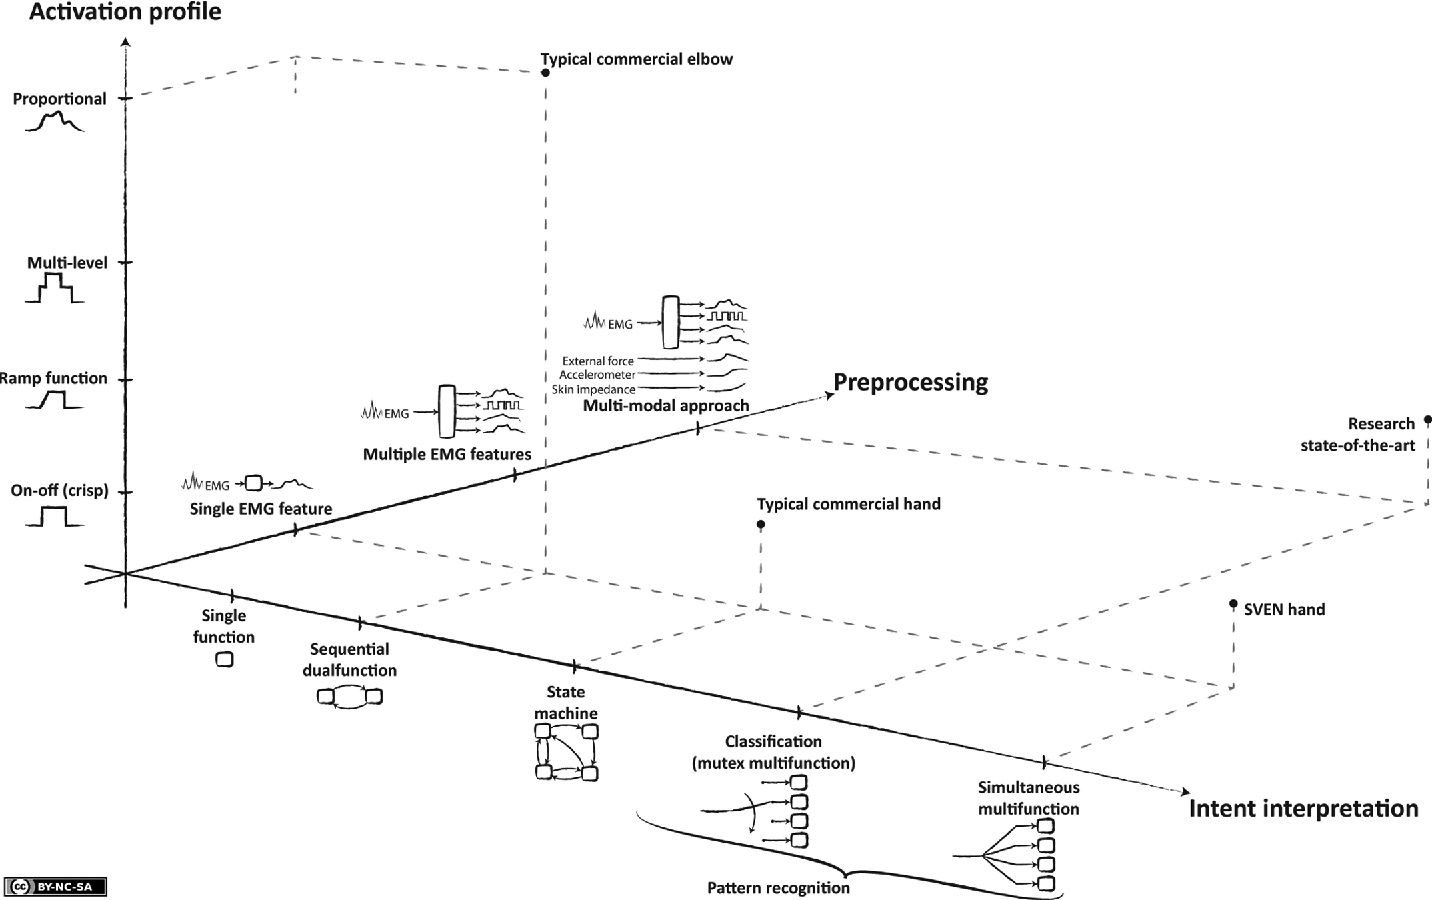
\includegraphics[width=1\textwidth]{Images/myoelectric-control.png}
    \caption{Research state-of-the-art of myoelectric control in the year 2012 [\cite{Fougner2012ControlOU}]}
    \label{fig:myo-control-schema}
\end{figure}
Electromyography (EMG) is an electrodiagnostic technique for evaluating and recording the electrical activity produced by skeletal muscles [\cite{0736093400}]. EMG is performed using an electromyograph which detects the electric potential generated by muscle cells when they are electrically or neurologically activated.
This electric potential can be approximatively considered proportional to the force of the muscle activation.
Due to the preference for noninvasive prostheses, surface EMG (sEMG) signals have been used for the control of upper limb prostheses prosthetic devices since 1948, as testified in \cite{Zecca2002}.
The signal produced by the sEMG sensors are fed to machine learning methods in order to control the prostheses: different machine learning models are used in union to different numbers of sEMG sigmals in order to achieve different level of control on the prostheses. A graphical representation of the different control methods and level, considering also non-machine learning methods, can be found in figure \ref{fig:myo-control-schema}.
In this thesis we work on a myoelectric control system characterized by a \textit{proportional} activation profile, a \textit{simultaneous multifunction} intent interpretation and we consider as input \textit{single EMG features} from multiple EMG sensors.